\section{Oppgave 1}
\begin{figure}[H]
    \centering
    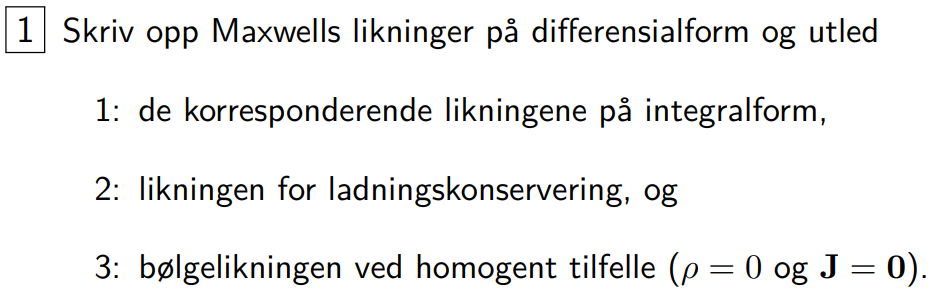
\includegraphics[width=0.7 \textwidth]{./01.png}
    \caption{}
    \label{fig:01}
\end{figure}


Maxwells likninger på differensialform er:

\begin{itemize}
    \item \textbf{Gauss' lov for elektrisitet:} $\nabla \cdot \vec{E} = \frac{\rho}{\epsilon_0}$. Denne loven beskriver hvordan en elektrisk ladning produserer et elektrisk felt. Her er $\vec{E}$ det elektriske feltet, $\rho$ er ladningstettheten, og $\epsilon_0$ er permittiviteten til vakuum.
    \item \textbf{Gauss' lov for magnetisme:} $\nabla \cdot \vec{B} = 0$. Denne loven sier at det ikke finnes noen magnetiske monopoler. Med andre ord, magnetiske feltlinjer har ingen begynnelse eller slutt.
    \item \textbf{Faradays lov:} $\nabla \times \vec{E} = -\frac{\partial \vec{B}}{\partial t}$. Denne loven er grunnlaget for elektromagnetisk induksjon, det vil si produksjon av elektrisk strøm i en ledning ved å endre det magnetiske feltet som omgir den.
    \item \textbf{Ampères lov:} $c^2\nabla \times \vec{B} =\frac{\partial \vec{E}}{\partial t} + \frac{\vec{J}}{\epsilon_0}$. Denne loven beskriver hvordan en strøm produserer et magnetisk felt. Her er $c$ lyshastigheten, $\vec{B}$ er det magnetiske feltet, $\vec{J}$ er strømtettheten, og $\epsilon_0$ er permittiviteten til vakuum.
\end{itemize}


\subsection*{1: De korresponderende likningene på integralform:}

Gauss' divergensteorem sier at volumintegralet av divergensen av et vektorfelt over et volum er lik flateintegralet av dette vektorfeltet over overflaten som avgrenser volumet. Dette kan skrives matematisk som:

\begin{equation*}
\int_V (\nabla \cdot \vec{F}) dV = \oint_S \vec{F} \cdot d\vec{s}
\end{equation*}

Her er $\vec{F}$ et vektorfelt, $V$ er volumet, $S$ er overflaten som avgrenser volumet, og $d\vec{s}$ er et infinitesimalt arealvektorelement på overflaten $S$.

Når det gjelder Gauss' lov for elektrisitet, er $\vec{E}$ det elektriske feltet og $\rho/\epsilon_0$ er divergensen av feltet. Å bruke Gauss' divergensteorem betyr å gå fra differensialformen $\nabla \cdot \vec{E} = \rho/\epsilon_0$ til integralformen

\begin{equation*}
\oint_S \vec{E} \cdot d\vec{s} = \frac{1}{\epsilon_0}\int_V \rho dV
\end{equation*}

Her er $\int_V \rho dV$ den totale ladningen innenfor volumet $V$, som vi kaller $Q_{\text{inn}}$.

På samme måte, når vi anvender Gauss' divergensteorem på Gauss' lov for magnetisme, går vi fra differensialformen $\nabla \cdot \vec{B} = 0$ til integralformen

\begin{equation*}
\oint_S \vec{B} \cdot d\vec{s} = 0
\end{equation*}

Dette betyr at det totale magnetiske fluks ut av ethvert lukket overflate er null, noe som tilsvarer det fysiske faktum at det ikke finnes magnetiske monopoler.

Stokes' teorem er et annet grunnleggende teorem innen vektoranalyse. Det knytter sammen et linjeintegral over en lukket kurve og et overflateintegral over en overflate som er avgrenset av denne kurven.

Matematisk kan det skrives som:

\begin{equation*}
\oint_C \vec{F} \cdot d\vec{l} = \int_S (\nabla \times \vec{F}) \cdot d\vec{s}
\end{equation*}

Her er $\vec{F}$ et vektorfelt, $C$ er en lukket kurve, $S$ er overflaten som er avgrenset av kurven, og $d\vec{l}$ er et infinitesimalt linjeelement langs kurven.

I sammenheng med Faradays lov representerer $\vec{E}$ det elektriske feltet og $-\frac{\partial \vec{B}}{\partial t}$ er rotasjonen av feltet. Ved å bruke Stokes' teorem, kan vi gå fra differensialformen $\nabla \times \vec{E} = -\frac{\partial \vec{B}}{\partial t}$ til integralformen

\begin{equation*}
\oint_C \vec{E} \cdot d\vec{l} = -\int_S \frac{\partial \vec{B}}{\partial t} \cdot d\vec{s}
\end{equation*}

Høyre side av likningen representerer endringen i magnetisk fluks gjennom overflaten $S$. Dette uttrykkes som $-\frac{d\Phi_B}{dt}$, som er endringen i det magnetiske fluks gjennom flaten $S$ med hensyn på tid.

Det vil si, integralformen av Faradays lov sier at en tidsvarierende magnetisk fluks gjennom en lukket løkke vil indusere en elektromotorisk spenning (EMF) rundt løkken, som er essensen av elektromagnetisk induksjon.

Ampères lov med Maxwells tillegg kan utledes til integralform ved bruk av Stokes' teorem. På differensialform er loven gitt som

\begin{equation*}
c^2\nabla \times \vec{B} =\frac{\partial \vec{E}}{\partial t} + \frac{\vec{J}}{\epsilon_0}
\end{equation*}

Ved å anvende Stokes' teorem kan vi konvertere det venstre uttrykket til et linjeintegral og det høyre uttrykket til et overflateintegral. Dette gir oss

\begin{equation*}
c^2 \oint_C \vec{B} \cdot d\vec{l} = \int_S \frac{\partial \vec{E}}{\partial t} \cdot d\vec{s} + \int_S \frac{\vec{J}}{\epsilon_0} \cdot d\vec{s}
\end{equation*}

Her er $C$ en lukket kurve, $S$ er overflaten avgrenset av $C$, $\vec{B}$ er det magnetiske feltet, $d\vec{l}$ er et infinitesimalt linjeelement langs $C$, $\vec{E}$ er det elektriske feltet, $\vec{J}$ er strømtettheten, og $d\vec{s}$ er et infinitesimalt arealvektorelement på overflaten $S$.

Integralformen av Ampères lov med Maxwells tillegg uttrykker forholdet mellom det magnetiske feltet rundt en lukket løkke og summen av den elektriske strøm som passerer gjennom løkken og den tidsderiverte av det elektriske fluks som passerer gjennom den samme løkken. Denne loven er grunnlaget for elektromagnetiske bølger.

Dette fullfører utledningen av Maxwells likninger på integralform fra differensialformen.

\subsection*{2: Ladningskonservering}
Ladningskonservering kan utledes fra Maxwells ligninger, spesielt fra Gauss' lov for elektrisitet og den korrigerte formen av Ampères lov.

Begynn med å ta divergensen på begge sider av Ampères lov:

\begin{equation*}
c^2 \nabla \cdot (\nabla \times \vec{B}) = \nabla \cdot \left(\frac{\partial \vec{E}}{\partial t} + \frac{\vec{J}}{\epsilon_0}\right)
\end{equation*}

Venstre side blir null siden divergensen av et rotasjonsfelt alltid er null. Vi sitter da igjen med

\begin{equation*}
0 = \nabla \cdot \left(\frac{\partial \vec{E}}{\partial t} + \frac{\vec{J}}{\epsilon_0}\right)
\end{equation*}

som kan omskrives til

\begin{equation*}
0 = \frac{\partial}{\partial t} (\nabla \cdot \vec{E}) + \nabla \cdot \vec{J}
\end{equation*}

Nå kan vi erstatte divergensen av det elektriske feltet med ladningstettheten ved hjelp av Gauss' lov for elektrisitet. Dette gir oss

\begin{equation*}
0 = \frac{\partial \rho}{\partial t} + \nabla \cdot \vec{J}
\end{equation*}

som er likningen for ladningskonservering, eller kontinuitetslikningen. Den uttrykker at endringen av ladning i et gitt volum pluss strømmen ut av volumet er lik null, noe som betyr at ladning er konservert.

\subsection*{3: Bølgelikningen i et homogent medium}
For å utlede bølgelikningen i et homogent medium der $\rho=0$ og $\vec{J}=0$, kan vi starte fra Faradays lov og Ampères lov med Maxwells tillegg:

\begin{equation*}
\begin{aligned}
\nabla \times \vec{E} &= -\frac{\partial \vec{B}}{\partial t} \quad \text{(Faradays lov)}\
\nabla \times \vec{B} &= \mu_0 \epsilon_0\frac{\partial \vec{E}}{\partial t} \quad \text{(Ampères lov med Maxwells tillegg)}
\end{aligned}
\end{equation*}

Hvis vi nå tar rotasjonen på begge sider av Faradays lov og bruker vektoridentiteten $\nabla \times (\nabla \times \vec{s}) = \nabla (\nabla \cdot \vec{s}) - \nabla^2 \vec{s}$, får vi:

\begin{equation*}
\nabla \times (\nabla \times \vec{E}) = -\frac{\partial}{\partial t} (\nabla \times \vec{B})
\end{equation*}

Da vi vet at $\nabla \times \vec{B} = \mu_0\epsilon_0\frac{\partial \vec{E}}{\partial t}$ og at $\nabla \cdot \vec{E} = 0$ siden $\rho = 0$, kan vi erstatte disse i likningen over for å få:

\begin{equation*}
\nabla (\nabla \cdot \vec{E}) - \nabla^2 \vec{E} = -\mu_0\epsilon_0\frac{\partial^2 \vec{E}}{\partial t^2}
\end{equation*}

Dette reduserer til:

\begin{equation*}
\nabla^2 \vec{E} = \mu_0\epsilon_0\frac{\partial^2 \vec{E}}{\partial t^2}
\end{equation*}

Dette er bølgelikningen for det elektriske feltet $\vec{E}$.

På en tilsvarende måte, ved å ta rotasjonen på begge sider av Ampères lov med Maxwells tillegg og bruke de samme vektoridentitetene, får vi bølgelikningen for det magnetiske feltet $\vec{B}$:

\begin{equation*}
\nabla^2 \vec{B} = \mu_0\epsilon_0\frac{\partial^2 \vec{B}}{\partial t^2}
\end{equation*}

Dermed har vi utledet bølgelikningene for et homogent medium der $\rho=0$ og $\vec{J}=0$.